\paragraph{Marking}

\begin{figure}[ht]
    \centering
    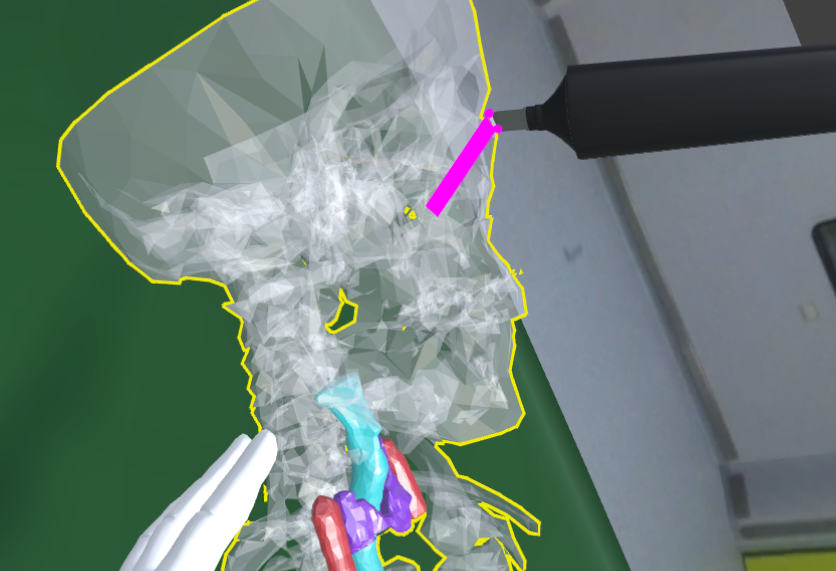
\includegraphics[width=200px]{images/implementation/features/procedures/marker.png}
    \caption{\label{fig::FeatureMarker}Marker Procedure}
\end{figure}

The \textbf{marking} procedure is similar to the bonesaw procedure, meaning that rectangular shapes are drawed into the three dimensianal space (Figure \ref{fig::FeatureMarker}).
However, here the created shapes are much thinner.
In contrast to the bonesaw, the virtual hands of the user are also disabled here.
This way, the user can decide to hold the marker in the optimal way.
Since the main objective is marking specific spots on the patient, this is the natural approach.